\documentclass[letterpaper,12pt]{article}
\usepackage[left=3cm,right=3cm,top=3cm,bottom=3cm]{geometry}
\usepackage{enumerate}
\usepackage{graphicx}
\usepackage{grffile}
\usepackage{float}
\usepackage[usenames]{xcolor}

\title{MATH-469 Project Checkin}
\author{Eric Biggers}

\begin{document}
\maketitle

The goal of my project is to implement an algorithm that can assemble a genome,
given a set of reads that came from it.  The key idea in the algorithm I am
implementing is the construction of a string graph where the edges are labeled
with DNA sequences and the vertices correspond to reads, and a path through the
graph corresponds to a set of reads that assemble together consistently.

I have implemented the initial stages of the algorithm.  Each step has been
implemented as a separate binary program.  This means that the overall assembly
process will iteratively transform the data (including the graph) on-disk into
the final assembly.  The currently implemented programs are:

\begin{itemize}
\item
	{\tt convert-reads}:  Imports and merges a set of reads
	into a concise binary representation.
\item
	{\tt compute-overlaps}:  Takes as input a set of reads and outputs all
	pairwise overlaps between reads of a minimum length specified by the
	{\tt --min-overlap-len} option.  The algorithm avoids a pairwise
	comparison of all reads by using a hash table to find reads sharing a
	seed.  Only exact overlaps are considered at this point.

\item
	{\tt print-overlaps}:  Prints a textual representation of a set of
	overlaps, given a file containing the overlaps in binary format.

\item
	{\tt remove-contained-reads}:
	Given a set of reads and the overlaps that were computed from them,
	finds all reads that are fully contained by another read and discard
	them, along with the corresponding overlaps.  If a pair of reads is
	identicaly, only one copy of the read is kept.

\item
	{\tt build-directed-string-graph}:
	Given a set of reads and the overlaps that were computed from them,
	build the {\bf directed} string graph that models the genome assembly.
\item
	{\tt build-bidirected-string-graph}:
	Given a set of reads and the overlaps that were computed from them,
	build the {\bf bidirected} string graph that models the genome assembly.

\item
	{\tt print-string-graph}:
	Prints a textual representation of a directed or bidirected string
	graph, or prints statistics about the graph.

\item
	{\tt transitive-reduction}:
	Given a string graph, remove edges $v \to x$ where there exist edges $v
	\to w \to x$, provided that $v \to x$ is labeled by the same sequence as
	that of $v \to w$ concatenated with $v \to x$.  This program currently
	only works on directed string graphs, but the bidirected case is in
	progress.

\item
	{\tt collapse-unbranched-paths}:
	Given a string graph, collapse chains of vertices that have in-degree 1
	and out-degree 1.  This program currently only works on directed string
	graphs, but the bidirected case is in progress.

\item
	{\tt digraph-to-bidigraph}:
	Convert a directed string graph into a bidirected string graph.

\end{itemize}

The modular design allows for multiple possible data flows, but a possible flow
is {\tt convert-reads} $\to$ {\tt compute-overlaps} $\to$ {\tt
remove-contained-reads} $\to$ \newline {\tt build-directed-string-graph} $\to$ {\tt
transitive-reduction} $\to$ {\tt digraph-to-bidigraph}, which will produce a
transitively-reduced, collapsed bidirected string graph produced from overlaps
between non-contained reads.

Even with the final stages not implemented, the algorithm is already effective
when used on random genomes because with no spurious overlaps, the
transitively-reduced string graph is a chain of vertices with no branching,
which then collapses into a single edge in {\tt collapse-unbranched-paths}.
This is true even if the genome is 15 million random base pairs, given 100 bp
reads sampled uniformly from either strand with no errors.  (Such a genome takes
about 1 minute to assemble with maximum memory usage 1.8 GB, with the main time
and memory bottleneck being the {\tt compute-overlaps} program).

What follows is an explanation of the initial stages of the algorithm on
64-character genome and three r

\noindent
{\tt 1.}
{\tt \color{red} $\leftarrow$TGAGCTTAAGGCTTATCTATCTTCAGACGACA$\leftarrow$ }\\
{\tt 2.}
\hspace*{2.58cm}{\tt \color{red} $\leftarrow$TTATCTATCTTCAGACGACTATTATAGCGCGG$\leftarrow$}\\
{\tt G.}
{\tt $\leftarrow$TGAGCTTAAGGCTTATCTATCTTCAGACGACTATTATAGCGCGGCCAAGACTACGCGGAGCCCC$\leftarrow$} \\
{\tt G.}
{\tt $\rightarrow$ACTCGAATTCCGAATAGATAGAAGTCTGCTGATAATATCGCGCCGGTTCTGATGCGCCTCGGGG$\rightarrow$} \\
{\tt 3.}
\hspace*{5.16cm}{\tt \color{blue} $\rightarrow$TCTGCTGATAATATCGCGCCGGTTCTGATGCG$\rightarrow$}

\begin{figure}
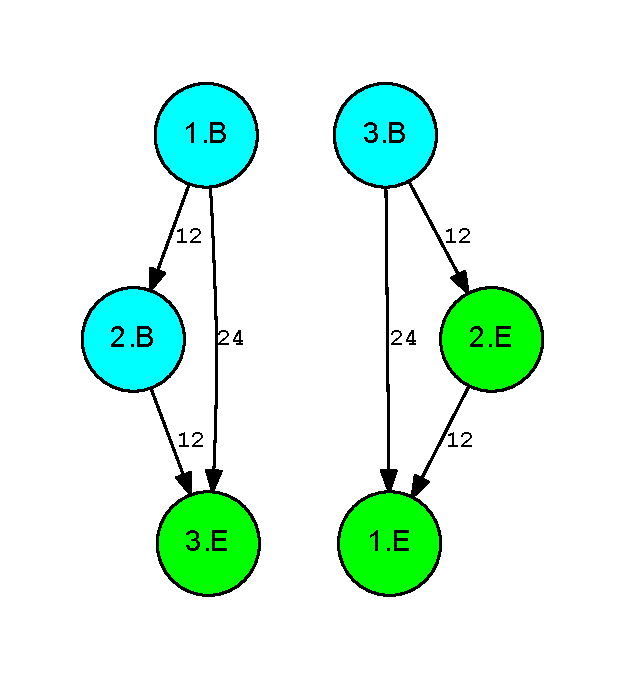
\includegraphics{out.digraph.pdf}
\end{figure}

\begin{figure}
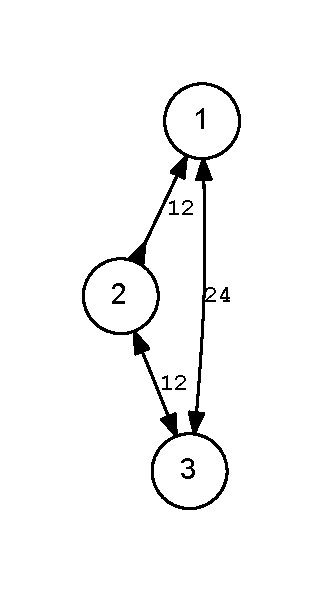
\includegraphics{out.bidigraph.pdf}
\end{figure}

\begin{figure}
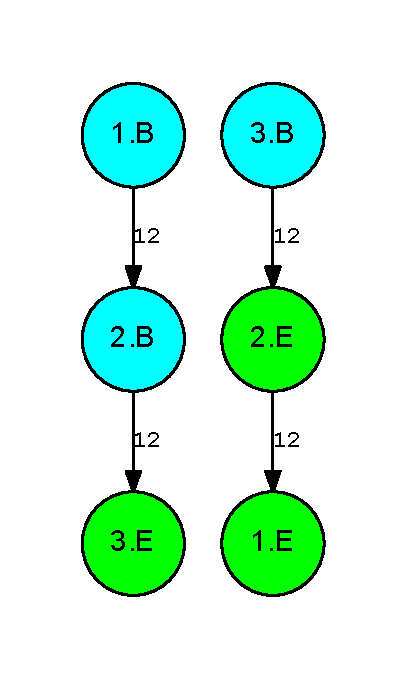
\includegraphics{out.reduced.digraph.pdf}
\end{figure}

\begin{figure}
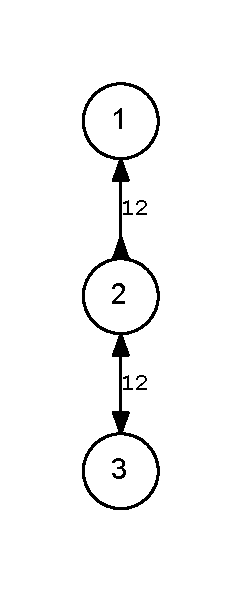
\includegraphics{out.reduced.bidigraph.pdf}
\end{figure}

\begin{figure}
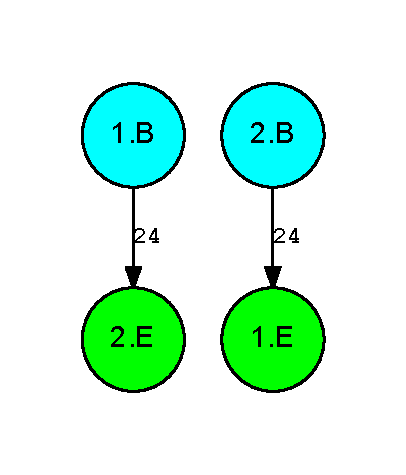
\includegraphics{out.reduced.collapsed.digraph.pdf}
\end{figure}

\begin{figure}
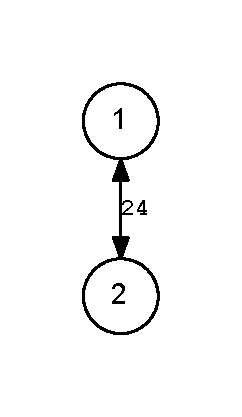
\includegraphics{out.reduced.collapsed.bidigraph.pdf}
\end{figure}

\end{document}
